% CONCLUSIONS
\chapter*{Synthèse et perspectives}
\markboth{Conclusions et perspectives}{}
\addcontentsline{toc}{chapter}{Conclusions et perspectives}
\newpage

L'étude des flux de carbone dans les écosystèmes tourbeux est complexe car assujetti à des facteurs de contrôle dont la prépondérance varie fortement selon l'échelle considérée et les conditions environnementales.

\section{Bilan du bilan (de C) ?}

Malgré tout les observations réalisées sur la tourbière de La Guette ont permis de mettre en évidence des flux de \coo particulièrement fort que ce soit pour la RE ou la PPB.
Cette force des flux de \coo est probablement liée à sa situation géographique locale et globale : une tourbière de plaine située à basse latitude et à ses problématiques de drainage et d'envahissement par une végétation vasculaire.
Ainsi la saisonnalité plus faible qu'en montagne permet aux flux de rester fort pendant une période de l'année plus importante.
Ces flux importants entraînent des variations forte en terme de bilan selon les méthodologies employées, il est cependant probable que la tourbière de La Guette fonctionne actuellement comme une source de carbone.

%L'estimation du bilan à l'échelle saisonnière ne permet pas de reproduire les variations journalières, l'estimation du modèle pendant les 3 jours de mesures haute fréquence réalisés en 2013 est largement supérieure aux valeurs mesurées (Figure~\ref{fig:RE1_vs_JN})

La prise en compte de la végétation reste une difficulté importante, l'observation répétée nécessitant des mesures non destructives, souvent imprécises ou très coûteuses en temps.
Paradoxalement les zones de la tourbières fonctionnant en puits de carbone sont celle ou les herbacées sont dominantes.

\subsection{RE : modélisation vs mesures}

Les estimations des flux de la tourbière de La Guette par les modèles du chapitre~\ref{ch:ch3} peuvent être comparé aux données acquises sur le même site lors d'autres expérimentations.
Ceci notamment grâce à l'utilisation de méthodes de mesures identiques sur l'ensemble de ces travaux.
Ainsi si l'on compare la RE estimée à l'aide du modèle RE-1 (chapitre~\ref{ch:ch3}) aux données acquises à haute fréquence (chapitre~\ref{ch:ch5}) on observe un écart important entre les valeurs mesurées et celles estimées par le modèle (Figure~\ref{fig:RE1_vs_JN}).
Pour expliquer cet écart on peut considérer les deux points suivants : 

Premier point, on compare un modèle qui prend en compte la variabilité spatiale du site (une partie au moins, à travers les vingts points qui on servi à calibrer le modèle) à des mesures réalisées sur quatre embases dans une zone restreinte de la tourbière (20 x \SI{20}{\metre}).
Ces quatre points ayant une représentativité spatiale limitée.
Cet écart peut donc être en partie le reflet de la variabilité spatiale des flux dans la tourbière.
Cet argument est soutenu par les mesures de RE réalisées le 24 et le 25 juillet 2013, soit 5 jours avant les mesures haute fréquence et dont la gamme de valeur est comprise entre \num{4.8} et \SI{18.9}{\uml} et sont représentés par le fond gris sur la figure~\ref{fig:RE1_vs_JN}.
Les estimations du modèle RE-1 restent d'ailleurs majoritairement dans cette gamme de valeurs.
Par ailleurs, la placette p04 (Figure~\ref{fig:carteVS}) la plus proche des mesures haute fréquences, est dans la gamme basse des flux que ce soit pour la campagne du 24-25 juillet : troisième flux le plus faible mesuré (\SI{6.1}{\uml}) ou en moyenne sur l'ensemble de mesure ou elle vaut \SI{2.81(160)}{\uml} par rapport à la moyenne de l'ensemble des placettes valant \SI{3.77(289)}{\uml}.

Second point, le modèle est calibré à partir de moyennes des flux par campagne de mesure (Figure~\ref{fig:ER_evolution_avg}).
Ces moyennes sont comprises entre \num{0.69(027)} et \SI{9.43(348)}{\uml}, par conséquent les estimations des modèles, dont RE-1, en dehors de cette gamme sont du domaine de l'extrapolation et donc à considérer avec précaution.

Ces deux points considérés, il semble que les estimations du modèle RE-1, malgré les écarts que l'on peut observées, restent cohérentes avec les mesures effectuées aux différentes échelles.
Cette comparaison montre également l'importance de la variabilité spatiale des flux dans les tourbières et la difficulté qu'il peut y avoir à la prendre en compte de façon satisfaisante.


\begin{figure}
\centering
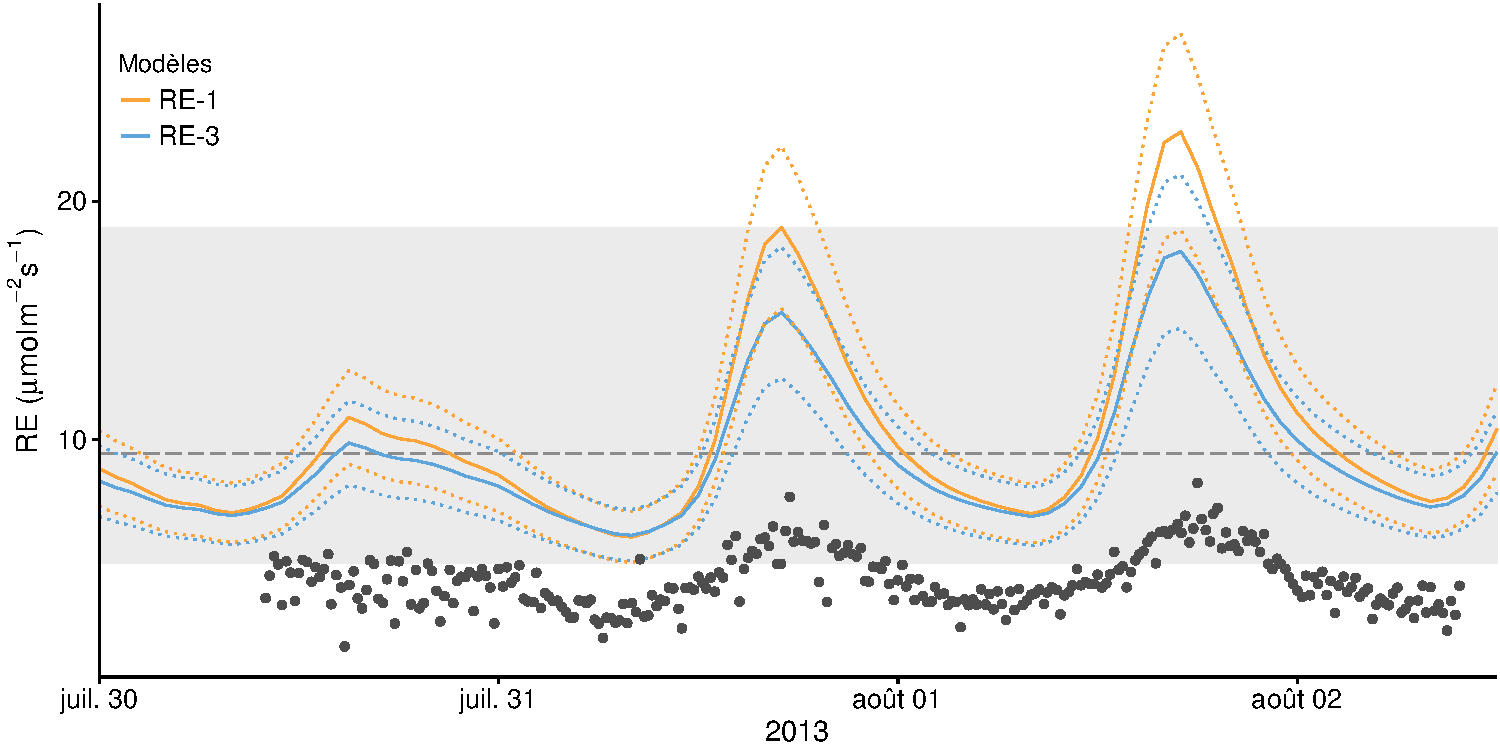
\includegraphics[width=\textwidth]{conclusions/RE1_vs_JN}
\caption{Comparaison entre les valeurs estimées par le modèle RE-1 et les mesures faites à haute fréquence sur le site du 30 juillet au 2 août 2013}
\label{fig:RE1_vs_JN}
\end{figure}


\section{L'hydrologie}

L'effet de la restauration hydrologique de la tourbière de La Guette n'a pas pu être mis en évidence de part une pluviométrie forte et un niveau de nappe toujours important.
Les expérimentations

\subsection{Résilience de la tourbe par rapport aux 2 années sèches qui précèdent le BdC}
(lien chap 3 et 4)

%schéma conceptuel ? Modèles globaux (ORCHID, chloée)
%
%Flux fort
%
%sensibilité param forte
%
%Modèles multi annuel et prise en compte de la végétation
%
%Quid des variations journalières dans un bilan annuel ? (Figure~\ref{fig:RE1_vs_JN})


Les prendre en compte améliorerait-il les modèles

modèles globaux ?
\textbf{limitations des équations :}
Plus généralement, la majorité des tourbières sont sous la neige une partie de l'année, ce qui n'arrive que rarement sur la tourbière de La Guette et une partie possède également des zones d'eau libre, qui n'existent pas sur ce site.

modèles globaux et profondeur de tourbe


\section{Ouverture vers d'autre méthodes de mesures}
\begin{itemize}
\item chambre automatique (lien chap 5, et chap 3 ?)
\item tour eddy covariance (lien chap 5 et chap 3 ?)
\end{itemize}

\section{perspectives}

La suite du projet CARBIODIV permettra peut être de mettre en évidence l'effet de la restauration.

Un partenariat avec le LSCE commencé pendant ces travaux devra permettre de valoriser ces données à des échelles plus importante.
Des données on d'ors et déjà été envoyée à Chloé XX qui développe un code "tourbière" dans le modèle ORCHIDEE.

L'installation prochaine d'une tour eddy covariance sur le site permettra de comparer ce bilan à des mesures plus haute fréquence.

\section{idées}

L'amélioration du protocole de végétation (RVI ?)

Amélioration des chambres (contrôle de la température ? de la vitesse du ventilateur ? plus grande ? aquisition automatisée du PAR sur la chambre)

l'inclusion des arbres

Correction du volume par pondération de la surface

Utilisation de chambres automatiques/EC

Humidité du sol

Propriétés physique de la tourbe (en cours)

